\section{Energy integration}


Nasibeh use cetow for heat puming solutions and st fons for large scale integration and combined heat and power production. We have to use neutralised values (i.e. we start with 100 unit and end up with 46.


Converting energy resources into useful energy, exergy efficiency, heat pumping and combined heat and power => examples from the papers of Nasibeh

adding a citation \cite{Pouransari_2014}

testing equations
\begin{equation}
min \, obj= \frac{things_{good}}{things_{bad}} \forall things\\
\text{subject to}  \\
things_{bad}\ge necessary\,\, level \cup unnecessary \, level
\end{equation}

**************

\subsection{Caste study I: Energy integration technologies}

The process heat transfer requirement for a real chemical site is identified using the data collected from different sources including energy conversion, distribution or process units. The heating and cooling requirements have been consequently determined. Based on the heating and cooling requirement definition, the Composite and the Grand Composite Curves are generated in \cref{fig1:mer}. It should be noticed that while defining the energy requirements, we have introduced the streams with the highest possible degree of freedom in order to target the greatest scope for improvement. An individual $\Delta T_{min}$ contribution is considered for each stream by adopting the typical value calculated from a predefined heat exchanger with the film heat transfer coefficient of each fluid at its relevant physical state. The Maximum Energy Recovery (MER) is then determined for the given $\Delta T_{min}$ and is considered as an initial target for heat recovery. \cref{fig1:mer}a shows the maximum heat recovery, the hot and the cold MER. The total heat requirement of the site is considered as the basis of 100\% unit here, and all the integration analysis values are based on this reference. In this case, there is a 54\% potential of integration (from the total heating requirement) compared to 40\% of integration in the current process which corresponds to the first ideal target.


        \begin{figure}[h]
        \begin{center}
        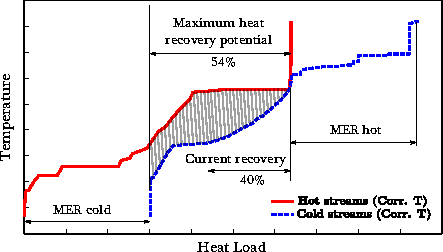
\includegraphics [height=4.3cm]{figures/EnergyIntegration/figMERcc.pdf} 
        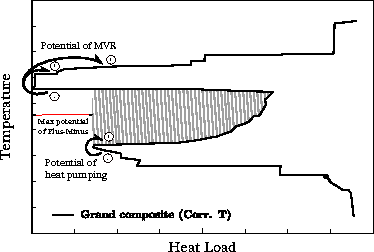
\includegraphics [height=4.3cm]{figures/EnergyIntegration/figMERgcc.pdf}
        \caption{Composite and Grand Composite Curves of the process after heat integration}
        \label{fig1:mer}
        \end{center}
        \end{figure}
        

Based on the result of the GCC and the plus-minus principle \cite{Linnhoff1993503}, the maximum heat recovery can be further improved by either integrating supplementary equipment (like the heat pump) or by modifying process operating conditions (such as modifying the pressure). The analysis of the GCC in \cref{fig1:mer}b with respect to the condition of this system (streams phase and temperature range) shows that there is a large potential for the Mechanical Vapor Recompression (MVR) or heat pumping (or both). The compression cycles are added to the appropriate place with respect to the pinch point temperature. This procedure is however possible until a new pinch point would be activated. Therefore, in order to increase the MVR potential while avoiding a quick creation of new pinch points, the heat pumping system is additionally proposed to be integrated with the Composite Curves. Considering the interdependency of the different actions, the flow rates and the selection of the most effective actions are obtained by solving an optimization problem. Obviously, we bear in mind that the implementation of every new solution of the system will modify the target. Suitable energy conversion units are now integrated and their optimum flow rate is found by Mixed Integer Linear Programming (MILP) formulation proposed by \citet{marechal1998process}. This formulation helps define the heat cascade of the Pinch Analysis method as a set of inequality constraints. This model selects the equipments in the superstructure and determines their optimal operating flow rate in the integrated system. The objective is then to minimize the operating costs, including the fuel and the electricity. In order to optimize the mass flow rates of the MVR, a new equality constraint is also added to the MILP optimization problem. The optimal integration of MVR and heat pumps is performed simultaneously with the energy conversion units. The Composite Curves of the system with MVR alone and together with the heat pumps are respectively shown in \cref{fig1:HPmvr}a and b. By adding an MVR unit, the mechanical power is calculated and a new hot stream is implemented. The principle of the calculation for the MVR is also reported in \cref{fig1:MVR}. In order to create a link between the part which is recompressed and the part used by the direct heat exchange, the equivalent of the expression $\left( \dot{m}_{total}=\dot{m}_{mvr}+\dot{m}_{dhe}\right) $ is added to the MILP problem as a new constraint \cite{EPFL-ARTICLE-163637}.


      \begin{figure}[h]
      \begin{center}
      \begin{tabular}{cc}
        \subfloat[With MVR]{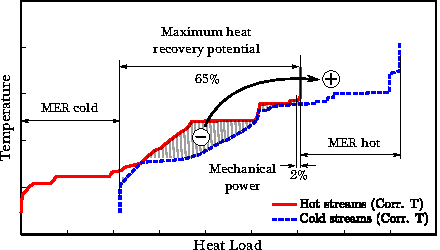
\includegraphics [height=4cm]{figures/EnergyIntegration/HPmvr_mvralone.pdf}} & 
        \subfloat[With MVR and HP]{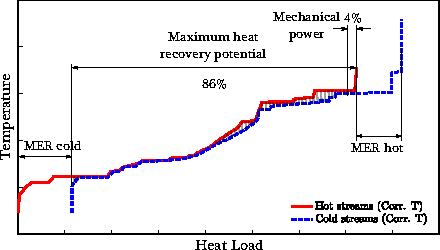
\includegraphics [height=4cm]{figures/EnergyIntegration/HPmvr_mvrhp.pdf}}
       \end{tabular}
      \caption{Composite Curves after improvement potentials}
      \label{fig1:HPmvr}
      \end{center}
      \end{figure}
      
      \begin{figure}[h]
 \begin{center}
 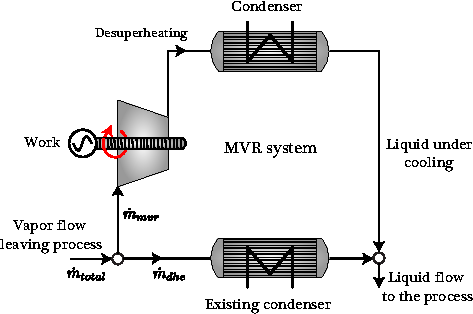
\includegraphics [width=80mm]{images/ch1/MVR.pdf}
 \caption{Principle of the MVR integration}
 \label{fig1:MVR}
 \end{center}
 \end{figure}
 
 Adding an MVR unit to transfer the heat from below to above of the pinch, results in the 11\% further improvement of the heat recovery potential (from 54\% in case of the process integration alone to 65\% in case MVR integrated) at the expense of 2\% mechanical power which corresponds to a COP of 5.5. Considering the newly activated pinch points in \cref{fig1:HPmvr}a, additional heat pumps are also added to system in \cref{fig1:HPmvr}b in order to further increase the heat recovery potential up to 86\%. This results to 32\% additional heat recovery than the original heat integration opportunities including 4\% of mechanical power requirement. This corresponds to a COP of 8. With the three ideal targets shown here, the overall evaluated energy savings could be between 20\% - 45\% approximately.
          
**************

\subsection{Caste study II: Site-Scale integration}

A large industrial process system can be analyzed by either \textit{Single Process Integration} (SPI) or through the \textit{Total Site Integration} (TSI). Both SPI and TSI lay on the same line in terms of approach, but in TSI the opportunity of heat recovery between the process systems is considered rather for the whole site than for each process system separately (SPI). In this case study, the SPI and TSI have been performed for the three process systems (Called as A, B and C) of a site by considering different representations***** for each process system. The total heat requirement of the site is considered as the basis of 100\% unit here, and all the integration analysis values are based on this reference. \cref{fig3:new} shows the repartition of the total consumption between the three process systems. It should be noticed that this 100\% unit does not define the heat consumption of the site cold streams because it considers the present heat recovery in the processes. The major consumers of each process system are identified such that 80\% of the total site consumption are considered in the analysis (Pareto principle). The remaining 20\% is therefore represented by black-box model and will not be considered for heat recovery in the analysis. 

\begin{figure*}[!ht]
\vspace{5mm}
\begin{center}
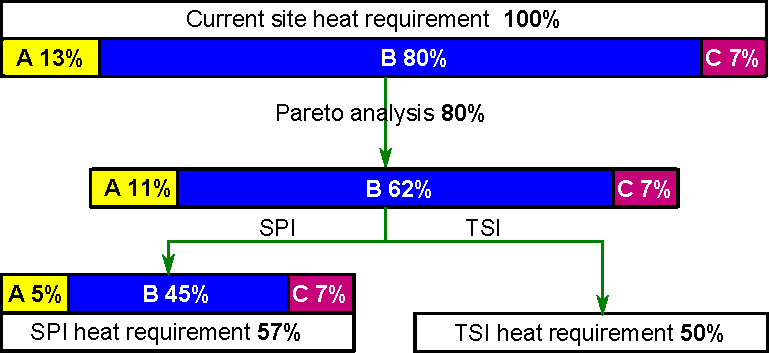
\includegraphics[width=125mm]{images/ch3/integrationAnalysis.pdf}
\caption{Summary of SPI and TSI for the three process subsystems of the site}
\label{fig3:new}
\end{center}
\end{figure*}

\subparagraph{Single Process Integration (SPI)}

The SPI is applied to each of the three process systems (\cref{fig3:III,fig3:IV,fig3:V}). The SPI analysis for the process system A is performed with a simple-model level***** of detail. 13\% of the total site consumption is explained by process system A, in which, after Pareto analysis, 11\% unit are considered in the integration analysis. The Composite Curves of this process system (\cref{fig3:III}b) show an increase for the potential of heat recovery from 2\% unit in the present situation, up to 8\% unit by integration. This means an energy saving of 62\% for the process system A, but only 7\% for the total site consumption. It should be noted that the 2\% unit heat recovery by P-P***** heat exchangers do not appear in the black-box model*****.

\vspace{10pt}
\begin{figure*}[!ht]
\begin{center}
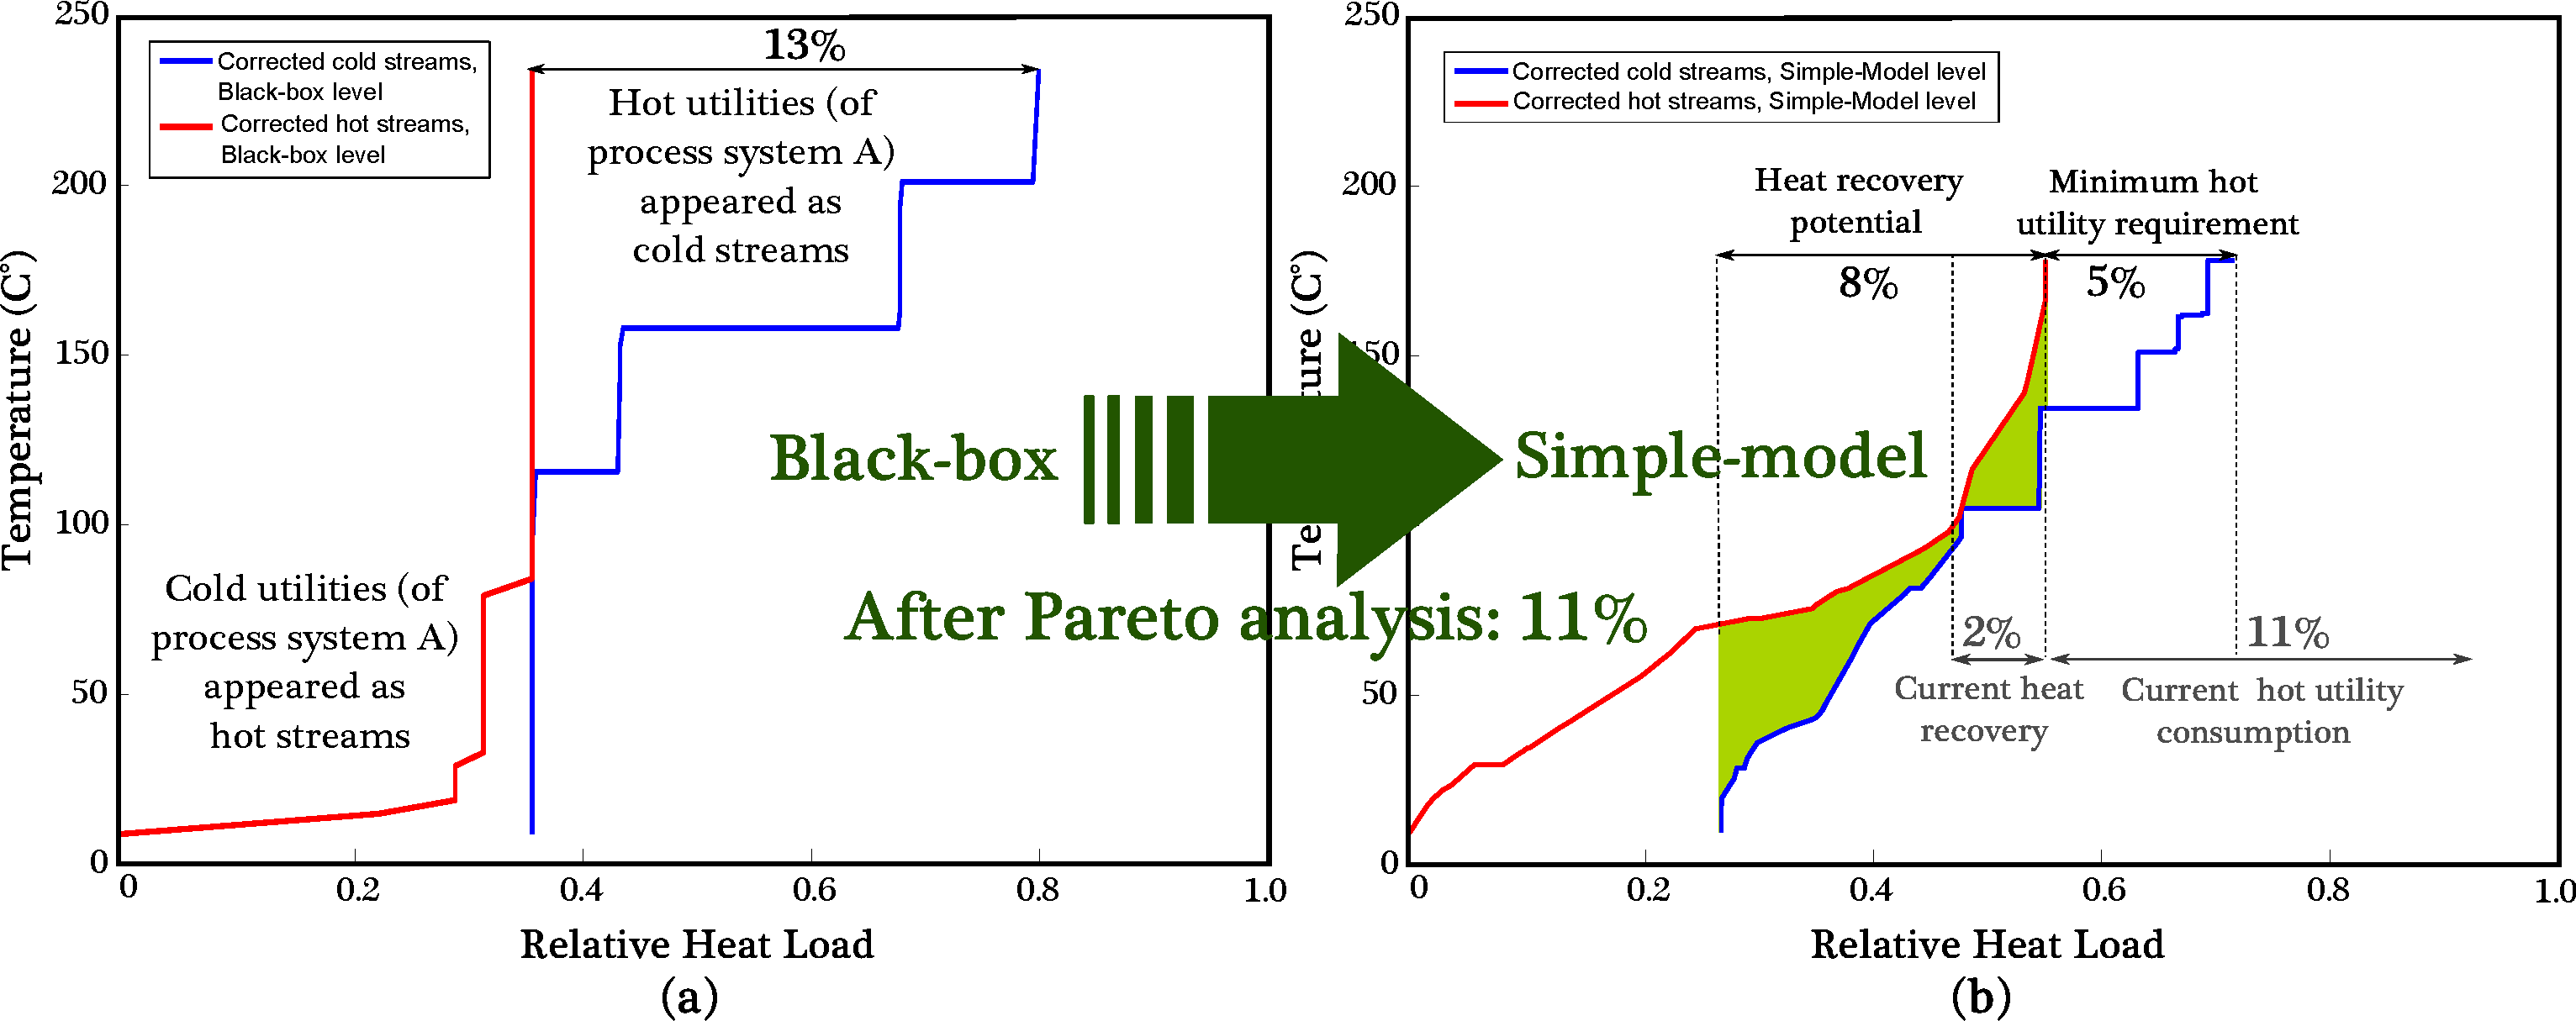
\includegraphics[width=146mm]{images/ch3/fig2ab.pdf}
\caption{Composite Curves of process system A from black-box to simple-model analysis with SPI (100\% corresponds to the present total site consumption)}
\label{fig3:III}
\end{center}
\end{figure*}

The same strategy is applied to the process system B, which represents 80\% of the whole consumption of the site. Since more detailed data were available from simulation model of this process system, the energy requirement analysis is using the detailed-model ****(\cref{fig3:IV}) that explains 62\% of the heat requirement after the Pareto analysis. The heat recovery potential is increased from 30 with the present heat exchangers, up to 47\% unit after integration. This corresponds to an energy saving of 17\% of the total site consumption or 19\% of process system B consumption.

 
\begin{figure*}[!ht]
\begin{center}
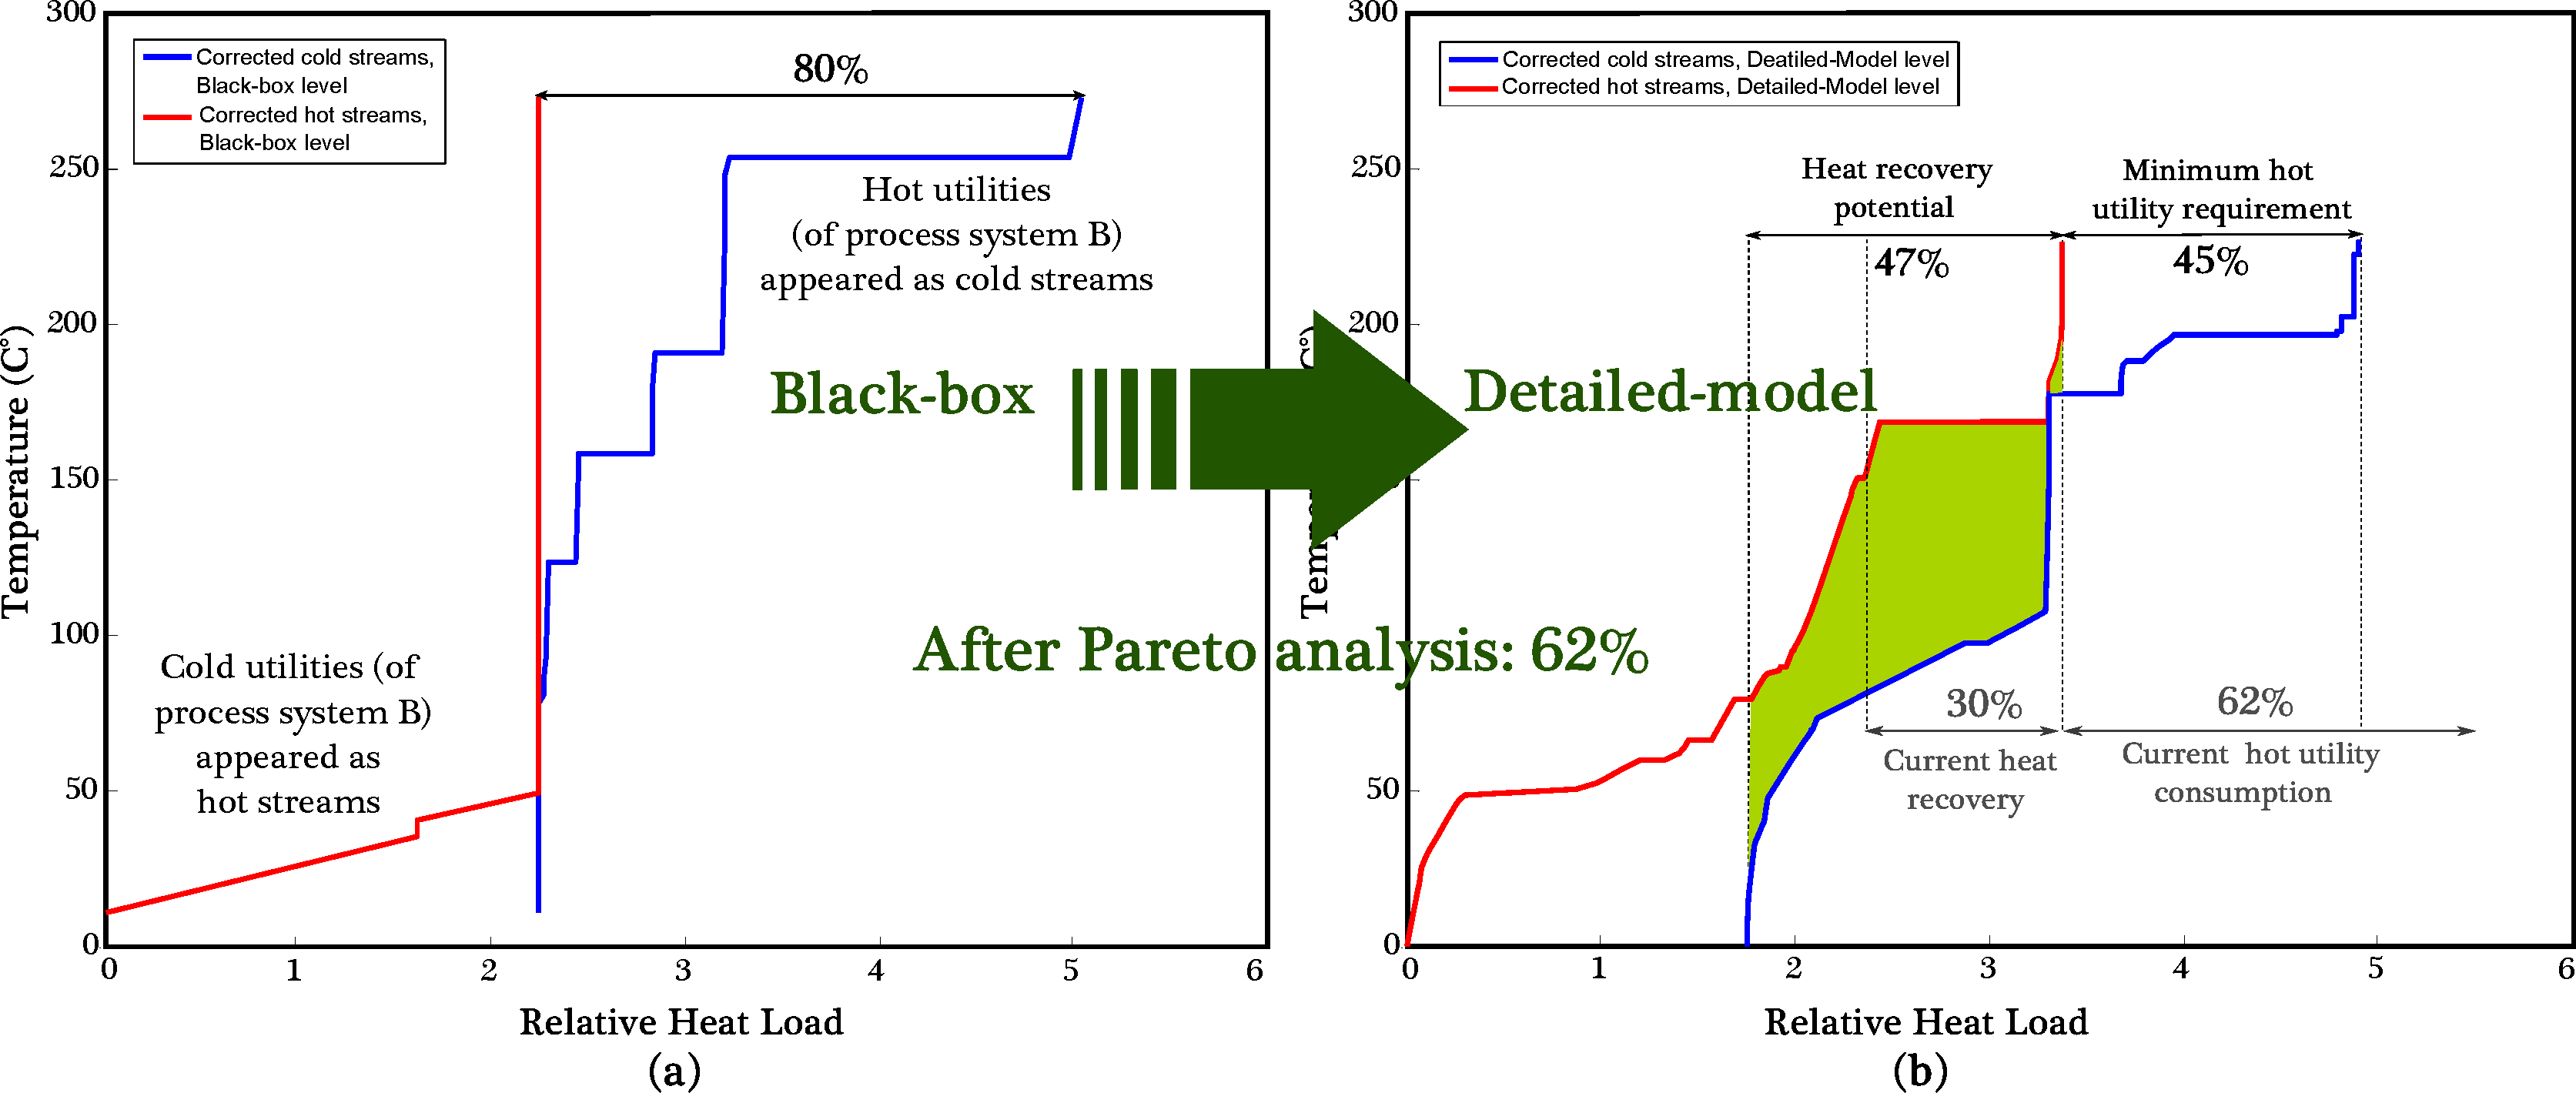
\includegraphics[width=146mm]{images/ch3/fig3ab.pdf}
\caption{Composite Curves of process system B from  black-box to detailed-model analysis with SPI (100\% corresponds to the present total site consumption)}
\label{fig3:IV}
\end{center}
\end{figure*}

Quite the opposite, the available data for process system C, which represents 7\% of the whole site heat consumption, is limited to the energy bill. It is therefore represented by the  black-box model***** (\cref{fig3:V}) and remains at the utility representation level**** ****.\footnote{This is another practical instance of how our multi-level data gathering procedure can come helpful to tune the analysis level of detail with respect to the available data} 
 
\vspace{10pt}
\begin{figure}[!ht]
\begin{center}
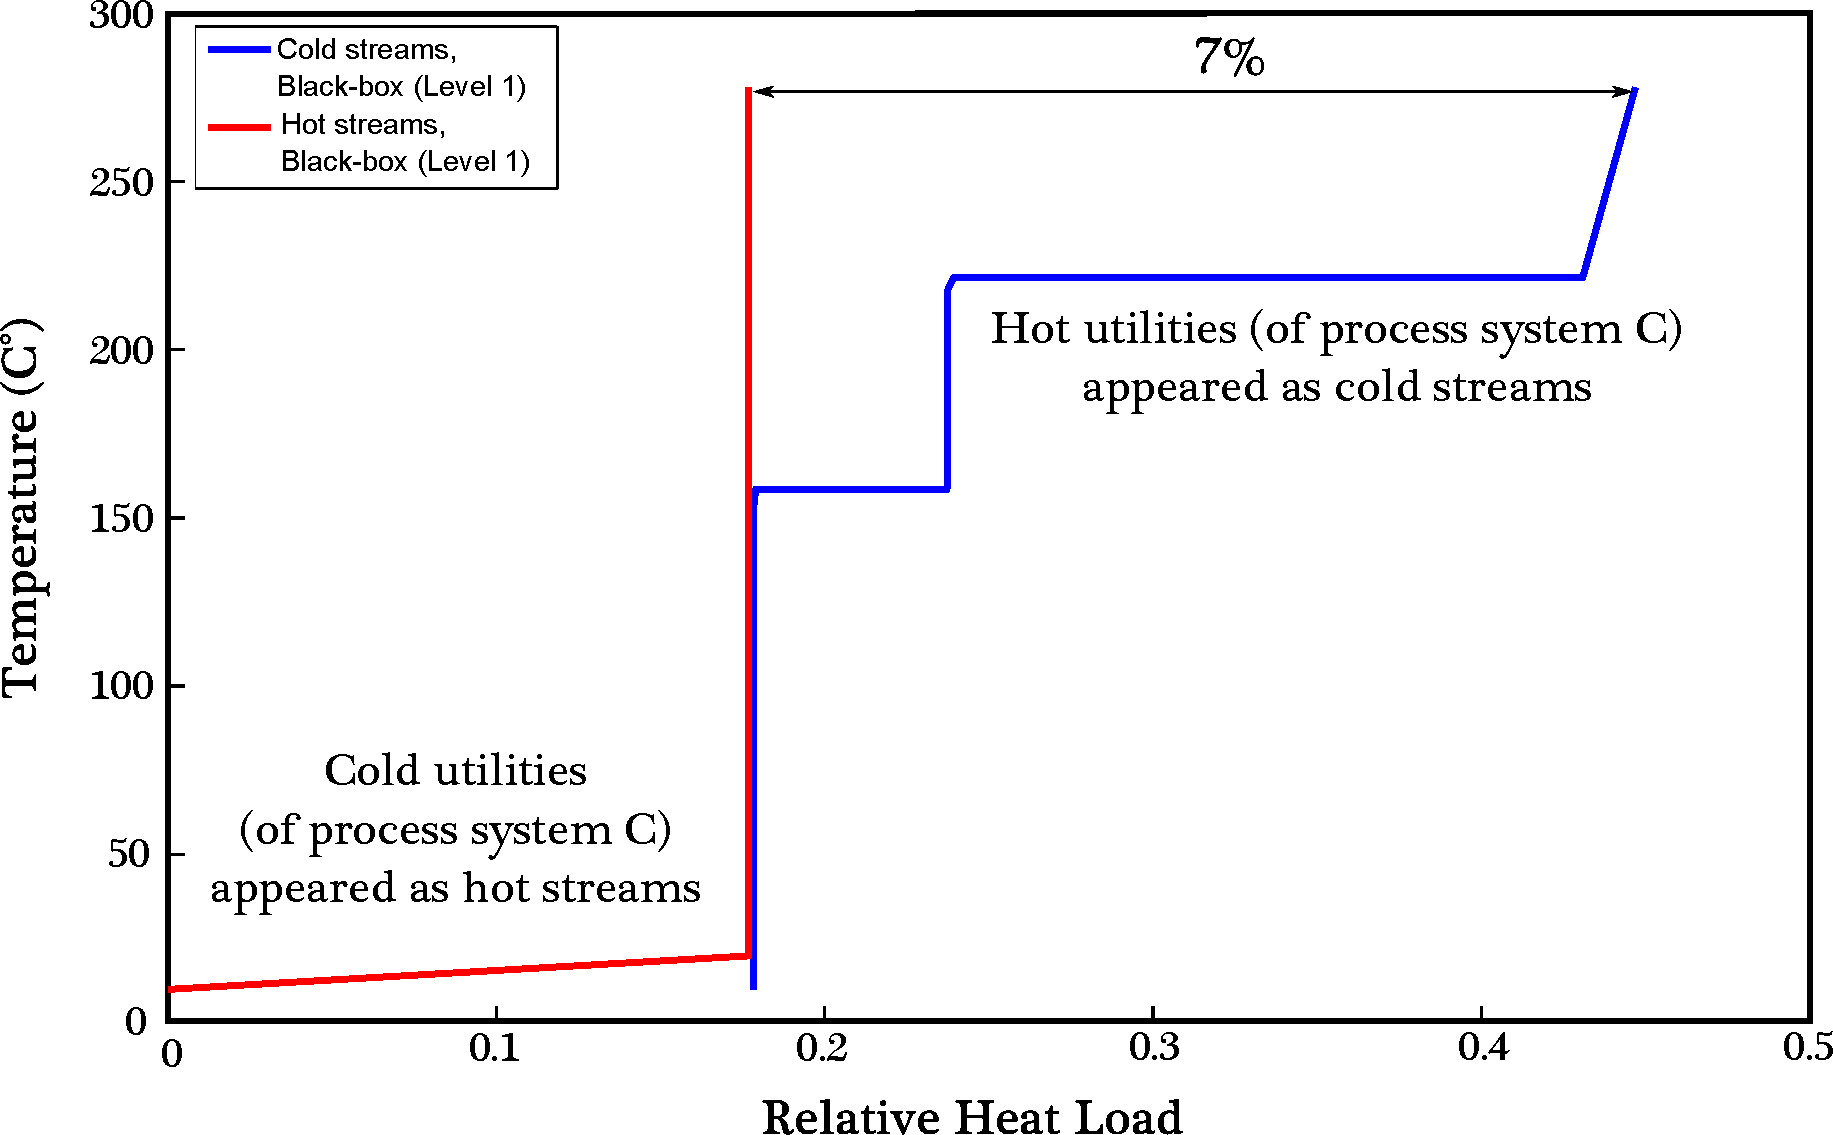
\includegraphics[width=80mm]{images/ch3/fig4.pdf}
\caption{Composite Curves of process system C with black-box analysis (100\% corresponds to the present total site consumption)}
\label{fig3:V}
\end{center}
\end{figure}

 Summing up the possible energy savings for the three process systems by SPI shows an additional heat recovery potential of 23\% unit. \cref{fig3:new} gives the detail of SPI analysis of the three process systems.
 
\subparagraph{Total Site Integration (TSI)}

In the TSI approach, combined with the multi-level energy requirement description, the first composite curves (\cref{fig3:VI}a) have been generated by applying the black-box analysis in which the utility representation of all process systems of the site is presented (after Pareto analysis). The result of this analysis gives a general overview of the current energy requirements of the site. However, the heat recovery potential cannot be pointed out with this representation. Consequently, the composite curves are systematically defined by upgrading the T-H profiles of the process systems with a more detailed requirement representation level.
 
 \begin{figure*}[!ht]
\vspace{5mm}
\begin{center}
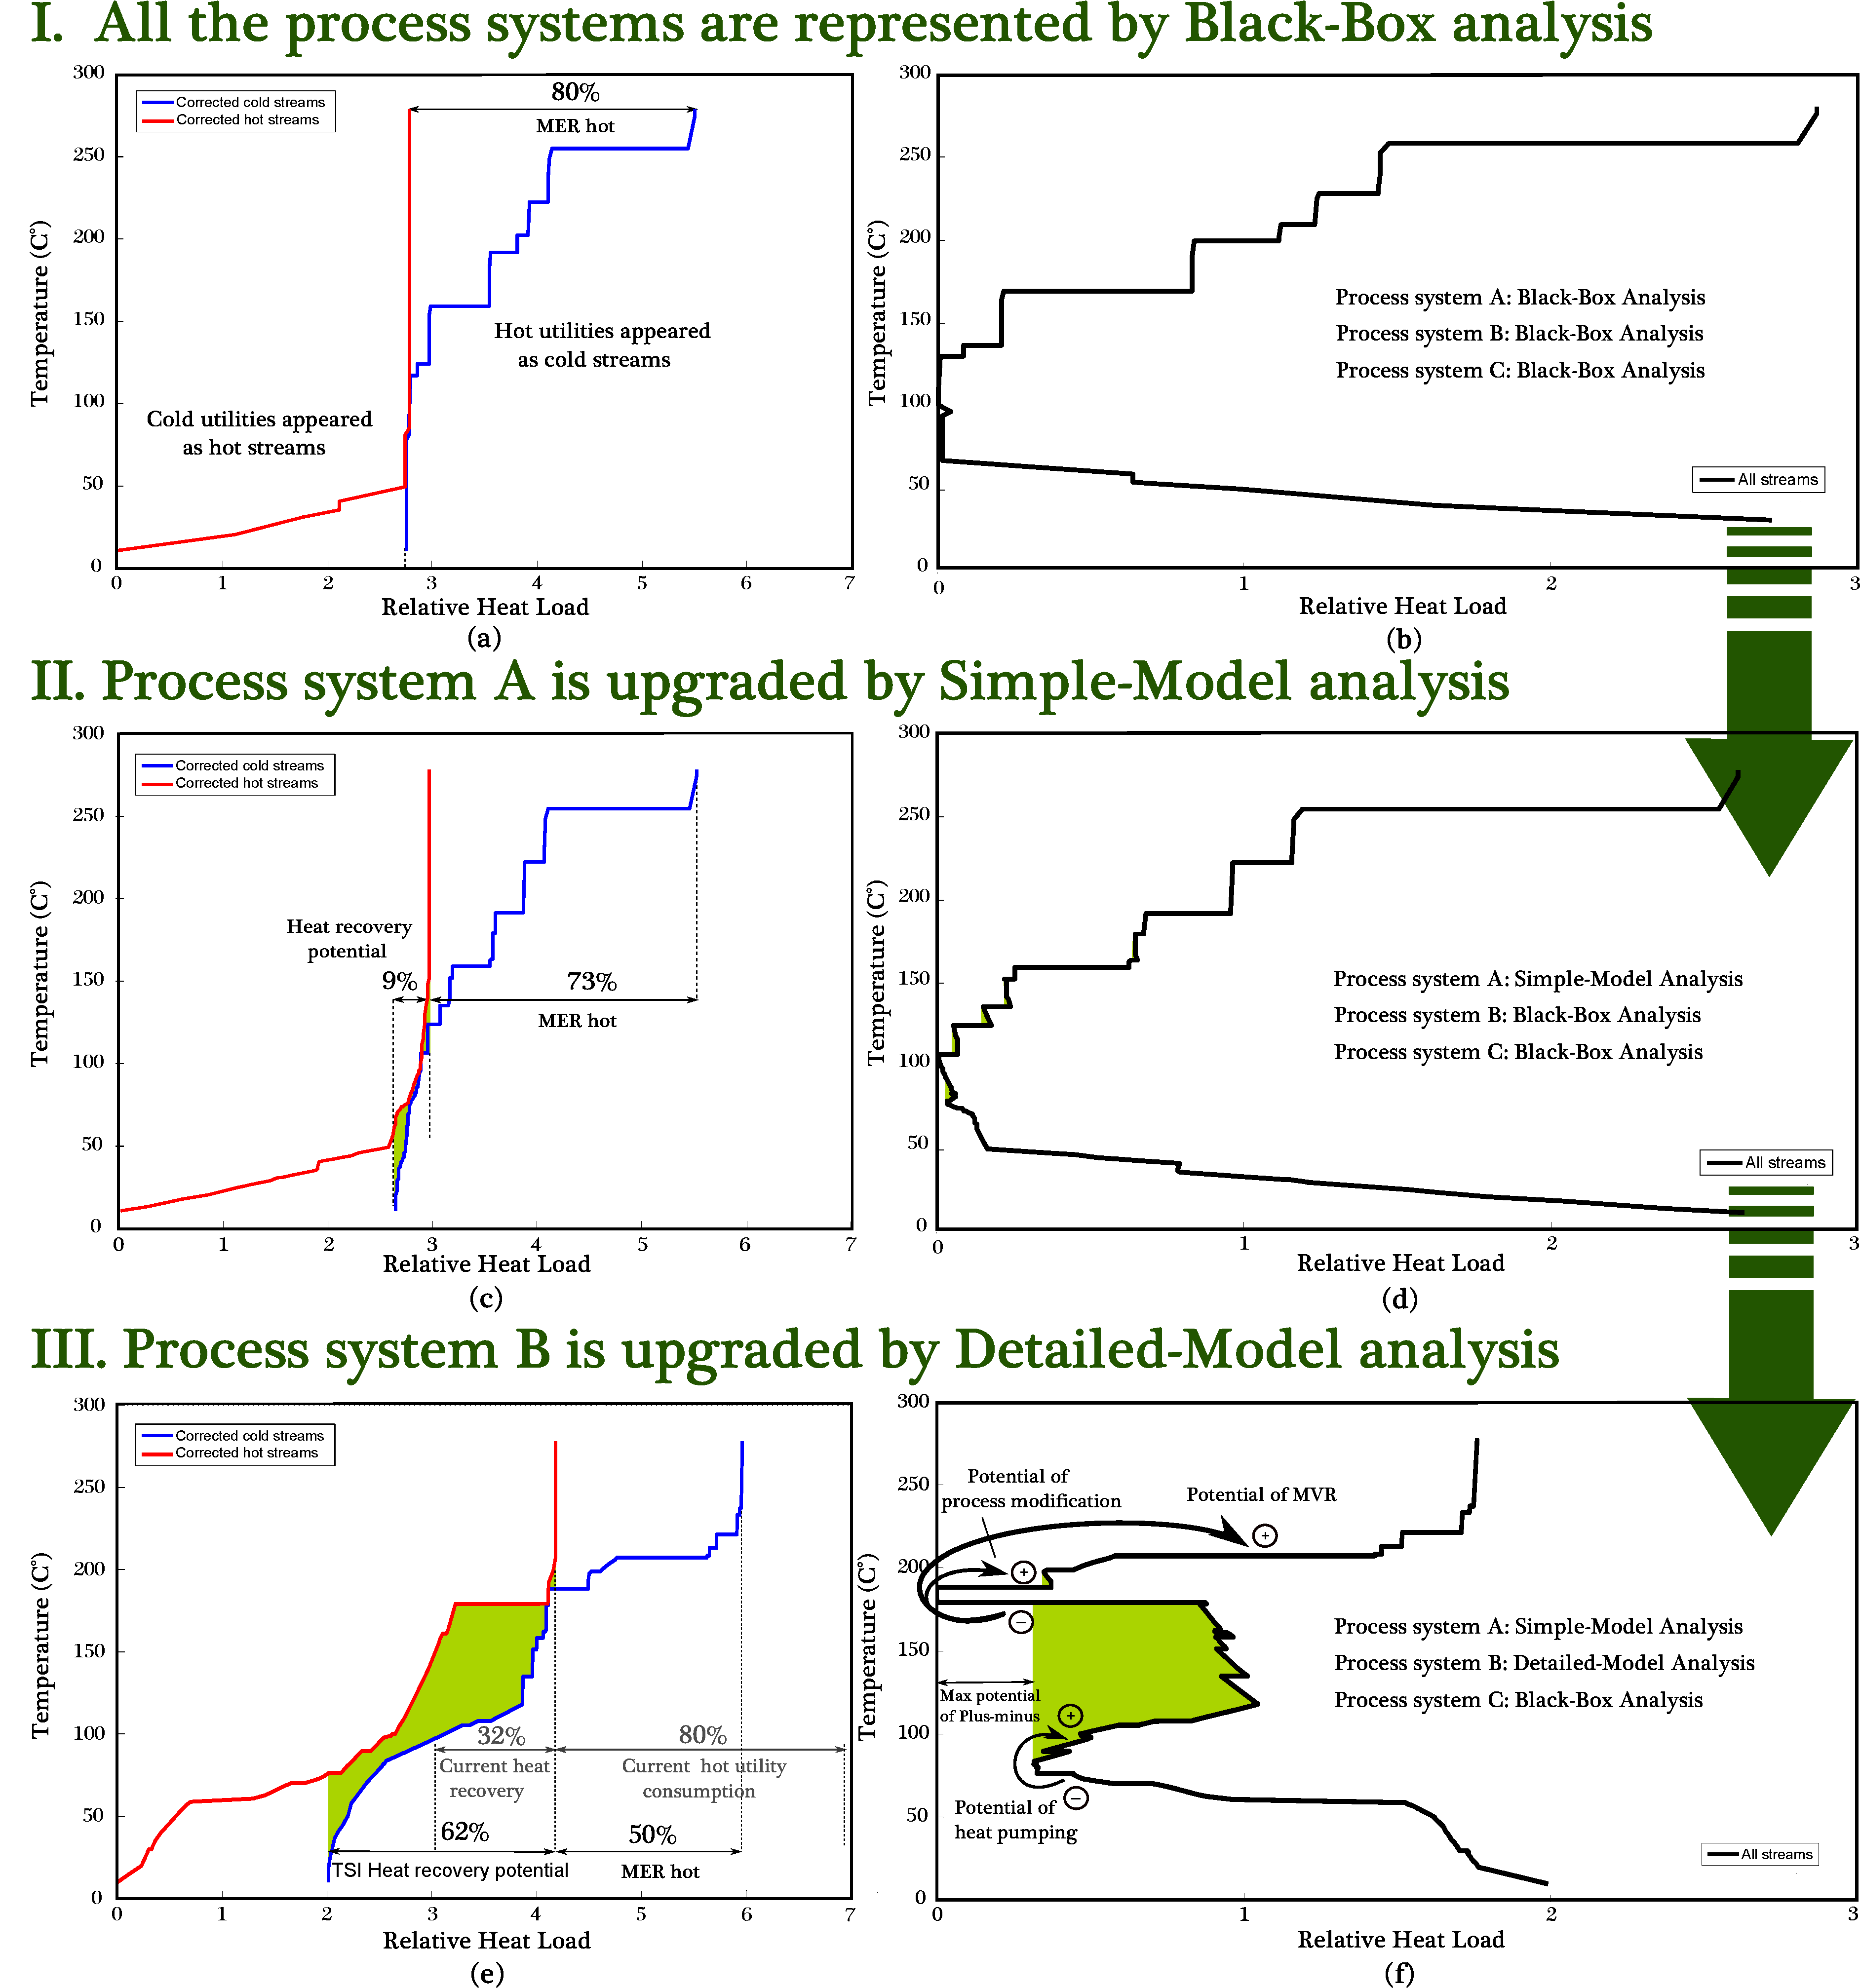
\includegraphics[width=146mm]{images/ch3/fig5.pdf}
\caption{Systematic improvement of Composite and Grand Composite Curves of total site by combining different energy requirement levels (100\% corresponds to the present total site consumption)}
\label{fig3:VI}
\end{center}
\end{figure*}

 \cref{fig3:VI}c shows the situation where the process system A has been represented by the simple-model while the other process systems remain with the utility representation. Upgrading the process system A from black-box to simple-model analysis, shows a heat recovery potential of 9\% unit that corresponds an additional 1\% unit recovered by exchanging heat between process system A and the other process systems. The analysis is continued by upgrading process system B from black-box to detailed-model (\cref{fig3:VI}e). The result of this integration shows that the total site heat requirement can be reduced to 70\% unit (50+20) which corresponds to 30\% energy saving. Comparing the result of TSI with SPI conclusion (Table. \ref{tab3:one}), exhibits 7\% unit more reduction in total heat requirement. This means that the heat requirement of the process system A (5\% unit) can be fully supplied by heat recovery with process system B. In addition, 2\% unit of process system C requirement can also be satisfied by heat recovery. The summary of SPI and TSI has been presented in Table. \ref{tab3:one}. 
 
 \subparagraph{Heat recovery improvement potentials}

With the analysis of the GCC of the site (\cref{fig3:VI}f) the maximum heat recovery can be further improved by either modifying the process operating conditions (increasing/decreasing the pressure of columns) or by adding supplementary equipment (MVR or HP). The purpose of all categories of modification is to move hot streams from  below to above the pinch or to move the cold streams located above the pinch to below the pinch (plus-minus principle). 

\begin{figure}[!ht]
\centering
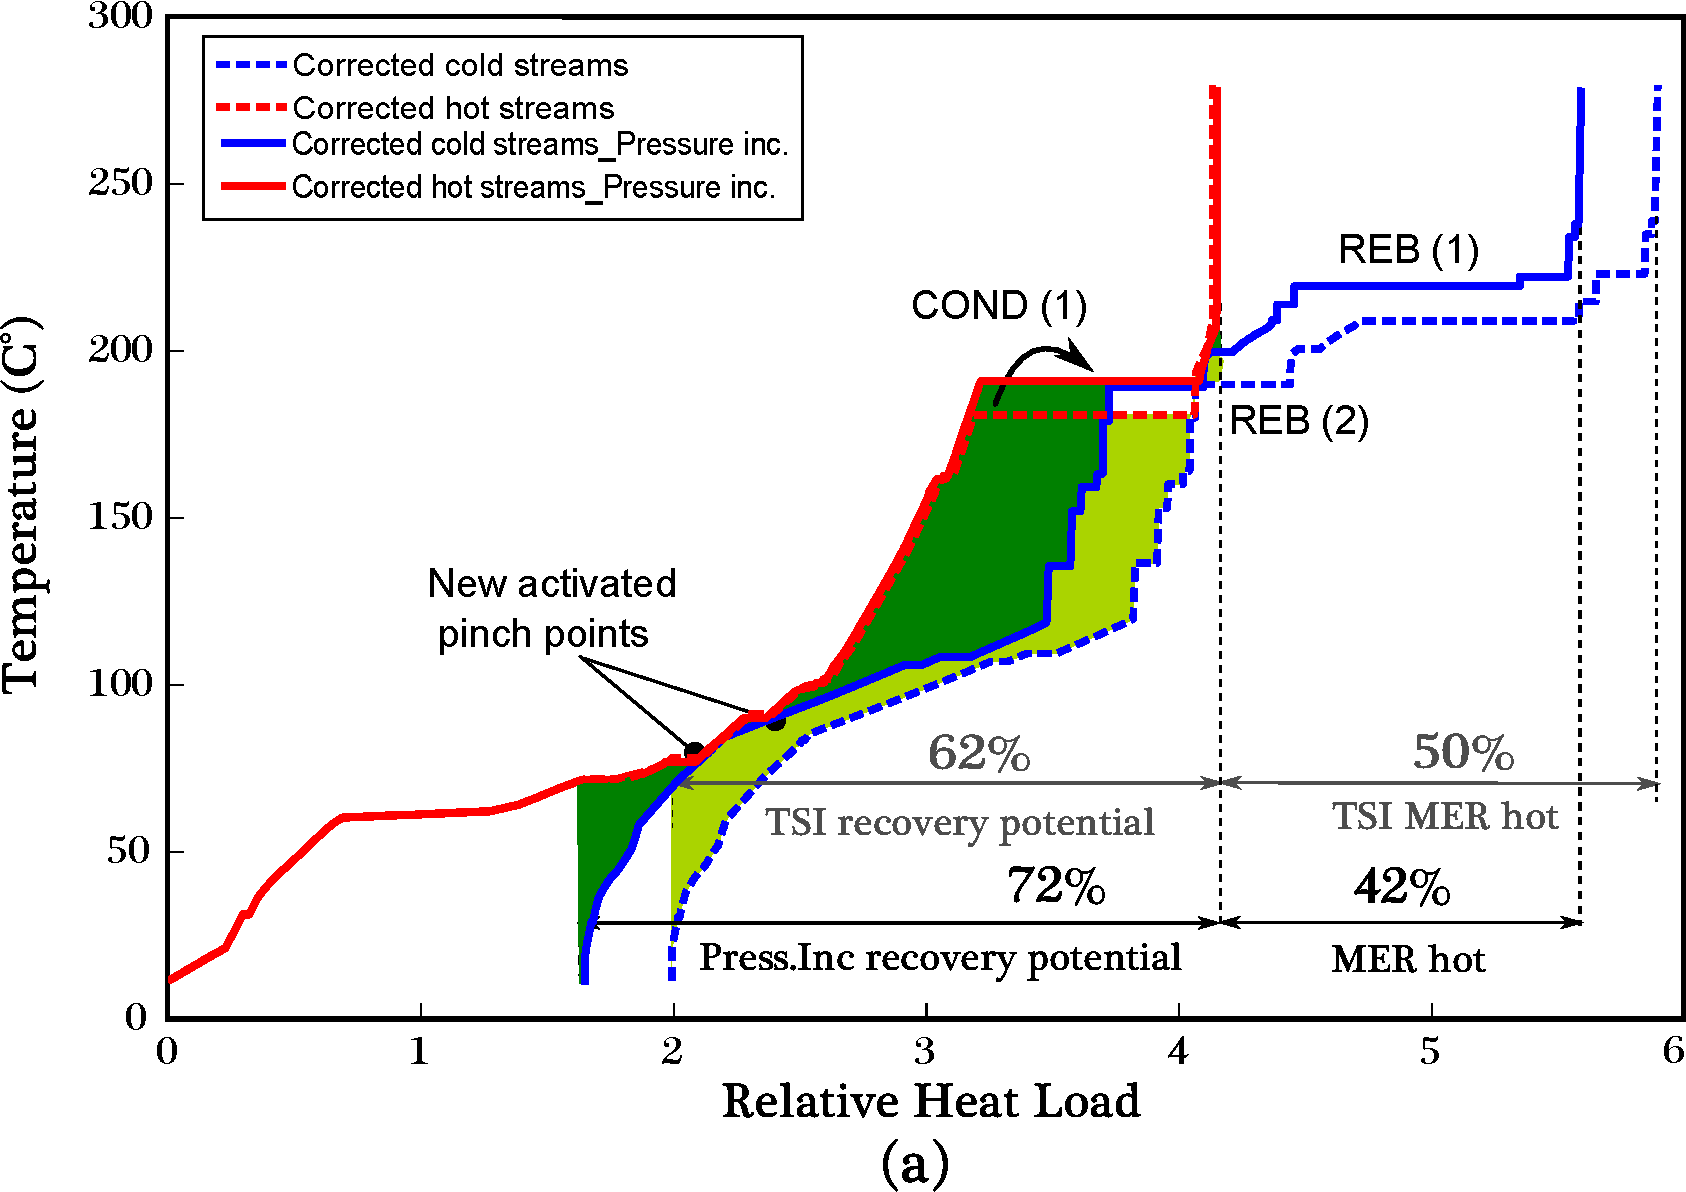
\includegraphics[width=71mm]{images/ch3/figpressa.pdf}
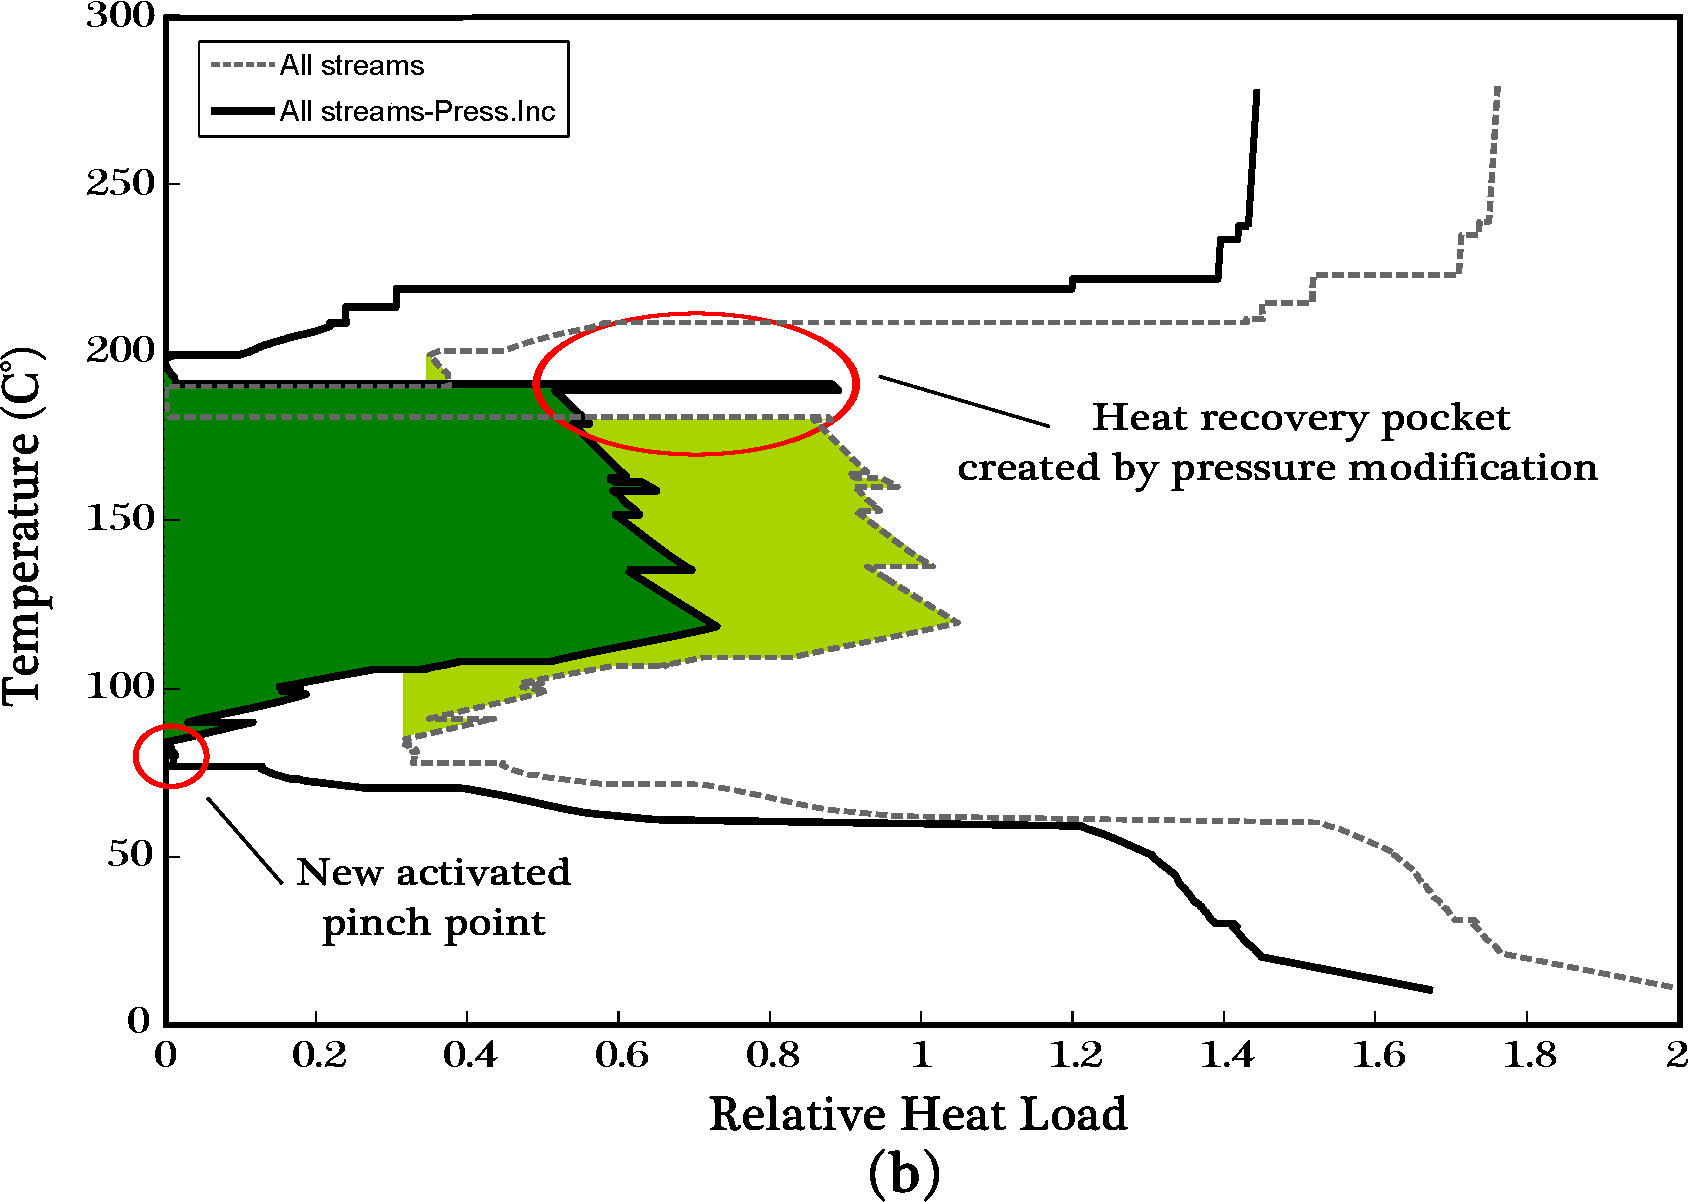
\includegraphics[width=70mm]{images/ch3/figpressb.pdf}
\caption{TSI for the process systems with and without pressure modification}
\label{fig3:VII}
\end{figure}

 Since the  streams that created the pinch are the condenser and reboiler of two distillation column units, the first proposition would be to modify the pressure of those columns. Therefore, the pressure of column (1) is modified ($\Delta p=0.4$ bar), in order to increase the temperature of its condenser up to above of the re-boiler of the column (2) (see \cref{fig3:VII}a). Consequently, the heat requirement is reduced by 8\% unit, therefore the overall hot MER is reduced to 42\% unit. Another possibility to upgrade the temperature of the condenser (1) above the re-boiler (2) is to apply heat pumping systems. The HPs can be implemented in two different ways: it can either be an HP with a closed cycle which uses an external fluid as a heat transfer intermediate, or an MVR which uses the process stream as a working fluid of the cycle. 
 
 \begin{figure}[!ht]
\centering
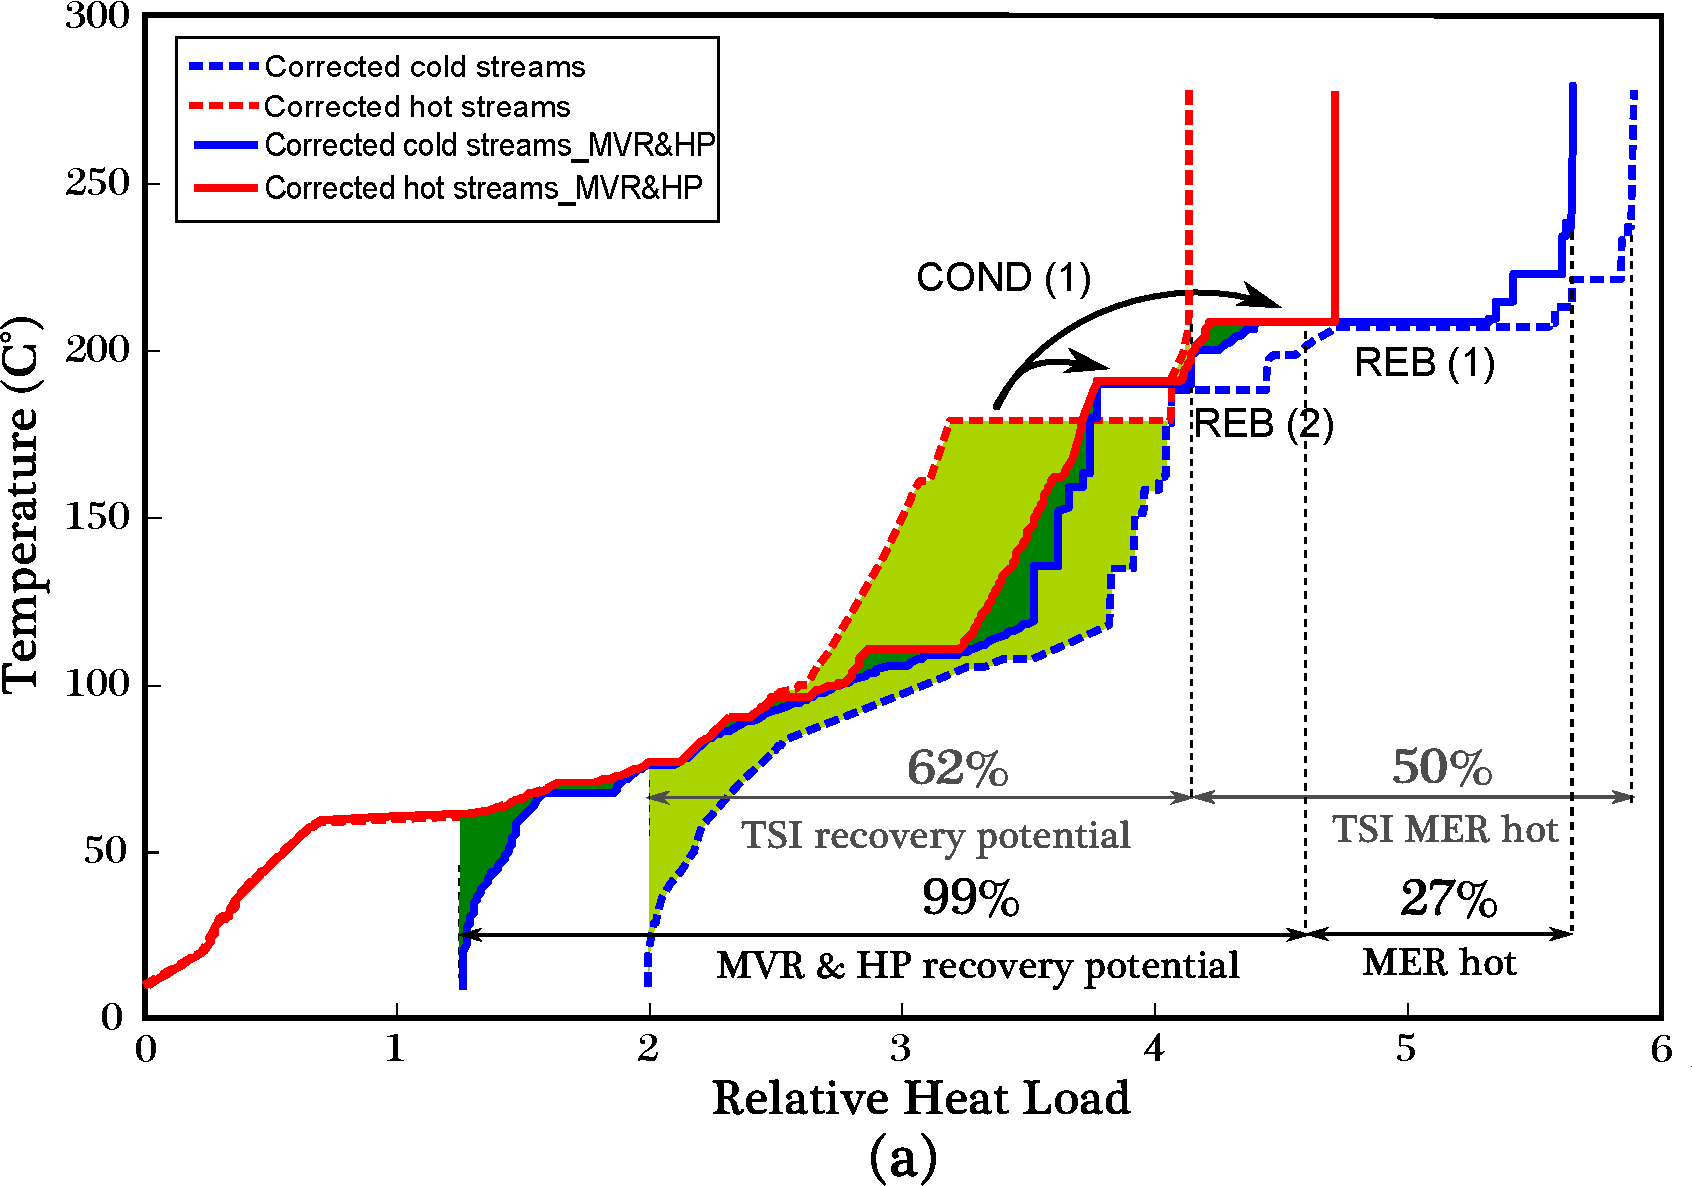
\includegraphics[width=71mm]{images/ch3/figmvra.pdf}
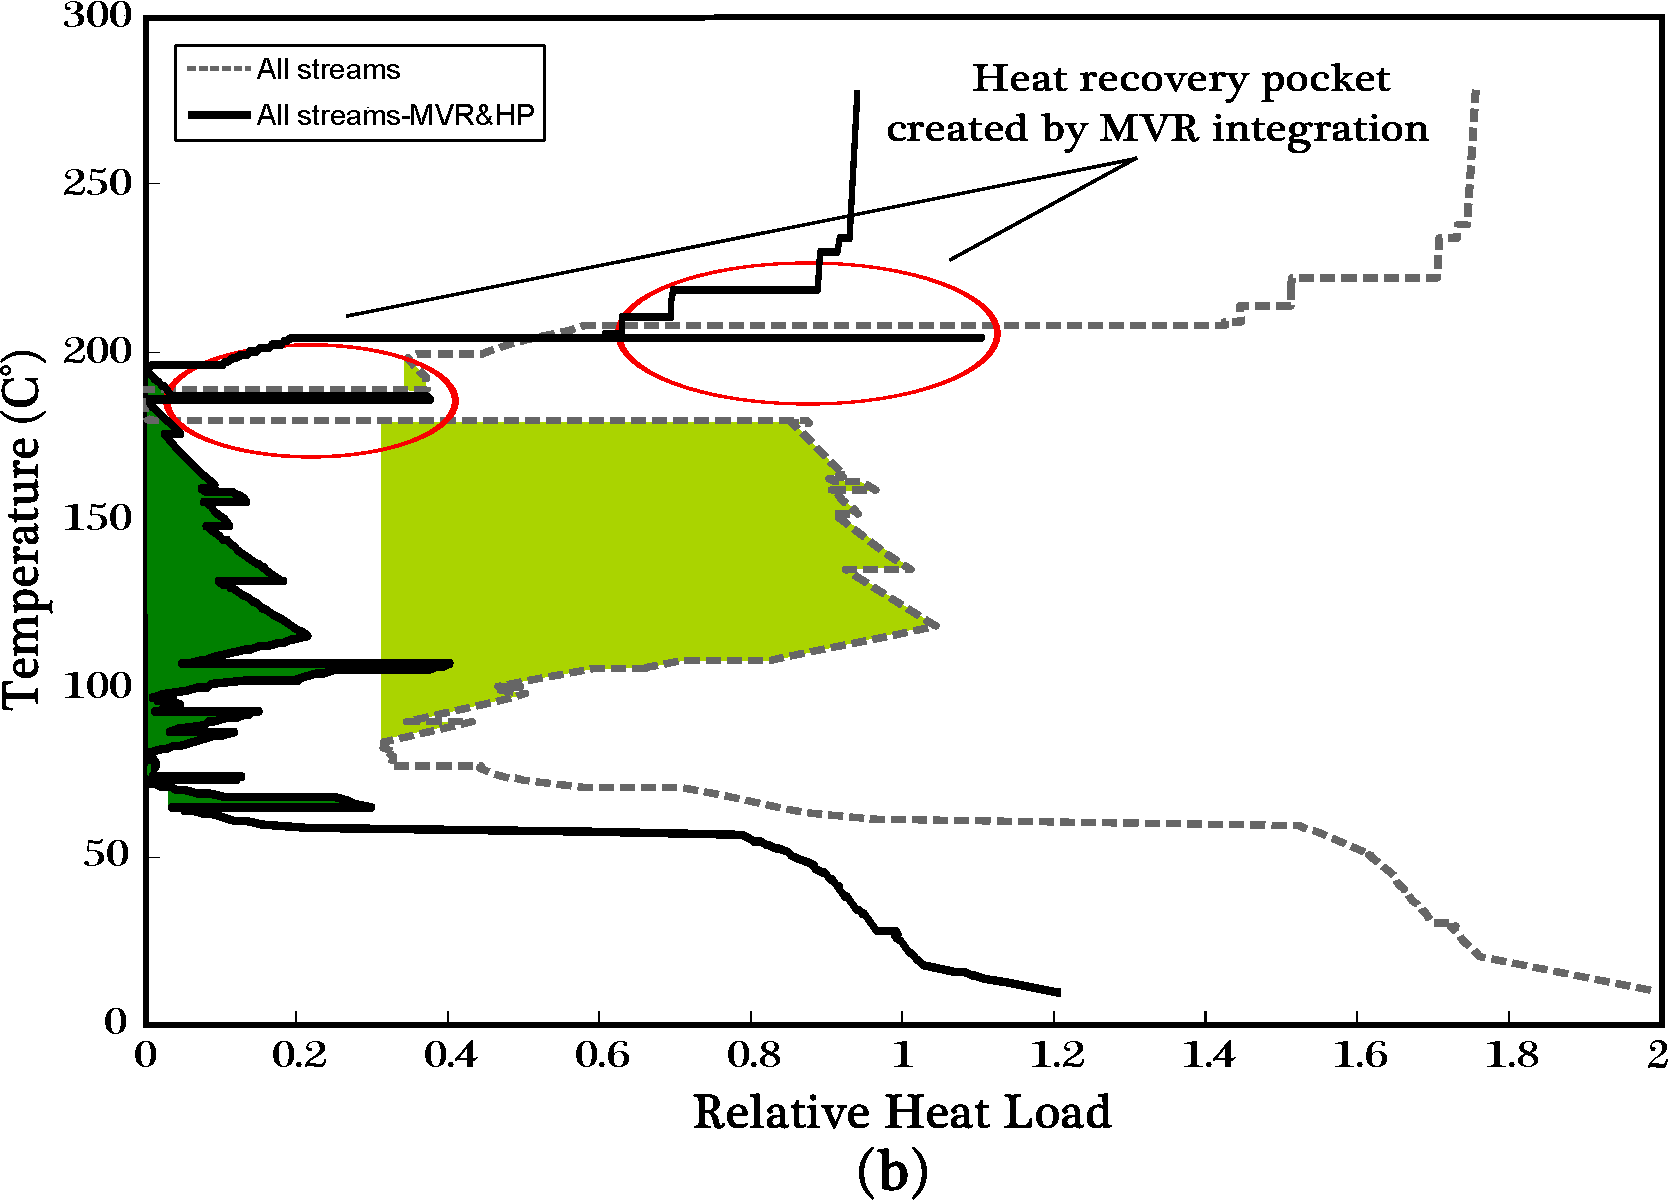
\includegraphics[width=70mm]{images/ch3/figmvrb.pdf}
\caption{TSI for the process systems with and without  MVR and heat pumps}
\label{fig3:VIII}
\end{figure}

 Considering the conditions of pinch streams (stream phases and temperature range), a multi-stage MVR is integrated to the column (1) in order to increase the temperature of the condenser (1) above of the re-boiler (1) and reboiler (2) (see \cref{fig3:VII}b). It should be mentioned that column (1) and (2) are in the same process system. Furthermore, in order to increase the recompression potential and also to avoid a quick creation of new pinch points, two HP systems are integrated to the lower edge of the composite curve. The heat requirement of the site is further reduced by 23\% unit with the integration of multi-stage MVR and HPs, for the expense of 6\% unit mechanical power requirement . The site energy bill is therefore reduced to 47\% unit (27+20). The optimal flow rates in the heat pumping system are obtained by optimization and integration simultaneously with the energy conversion unit. The optimal integration of MVR and HPs is therefore performed together with utility systems. 
 
 \subparagraph{Integration and optimization of energy conversion units}

 \cref{fig3:VIIII} shows the site utility integration and optimization results with Carnot factor representation\footnote{The ambient temperature ($T_0$) is assumed to be 25 $^{\circ}\mathrm{C}$ } for the three following scenarios: (a) base-case, (b) with pressure modification and (c) MVR and heat pumps integrated. The boiler, cogeneration unit with gas turbine, steam network with steam turbines and refrigeration cycle are the selected units within all three scenarios. One of the waste stream from the process is burned as a fuel in the boiler which creates 7\% unit of the current site heat requirement (0.2 relative heat load in \cref{fig3:VIIII}) and corresponds to the highest temperature level of utility streams. A gas turbine produces electricity with an efficiency of 33\% and produces a hot stream from 558 $^{\circ}\mathrm{C}$ to the stack temperature of 160 $^{\circ}\mathrm{C}$ with a thermal efficiency of 50\%. In the calculation, the part load efficiency of the gas turbine is not considered, however, the level of usage is verified to be consistent with its capacity. The price for different forms of energy, influences the choice of the appropriate technology and its level of usage in the integrated solution. Here, the ratio of gas price to the electricity is supposed to be $0.8$. The cogeneration unit is quite sensitive to the price of electricity and gas, thus in the presented solutions, the maximum capacity of the cogeneration system is optimized to produce an equivalent amount heat to the MER of each scenario. As a result, the electricity produced by the cogeneration unit, comes only from the excess exergy content of the necessary required gas that satisfies MER. 
 
  \vspace{5mm}
 \begin{figure}[!ht]
 \begin{center}
 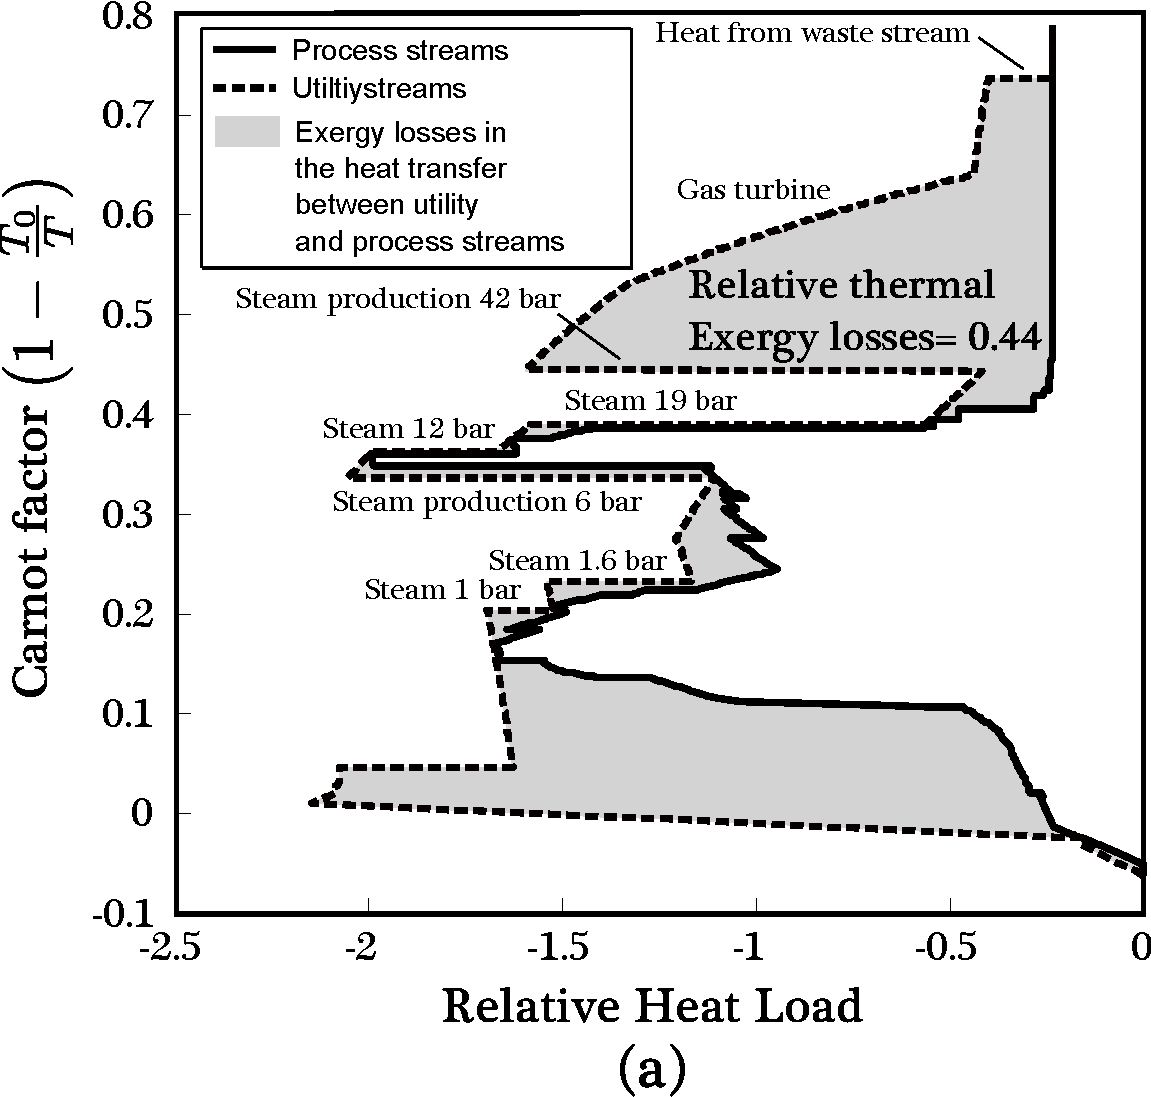
\includegraphics[width=70mm]{images/ch3/figutilitya.pdf}
 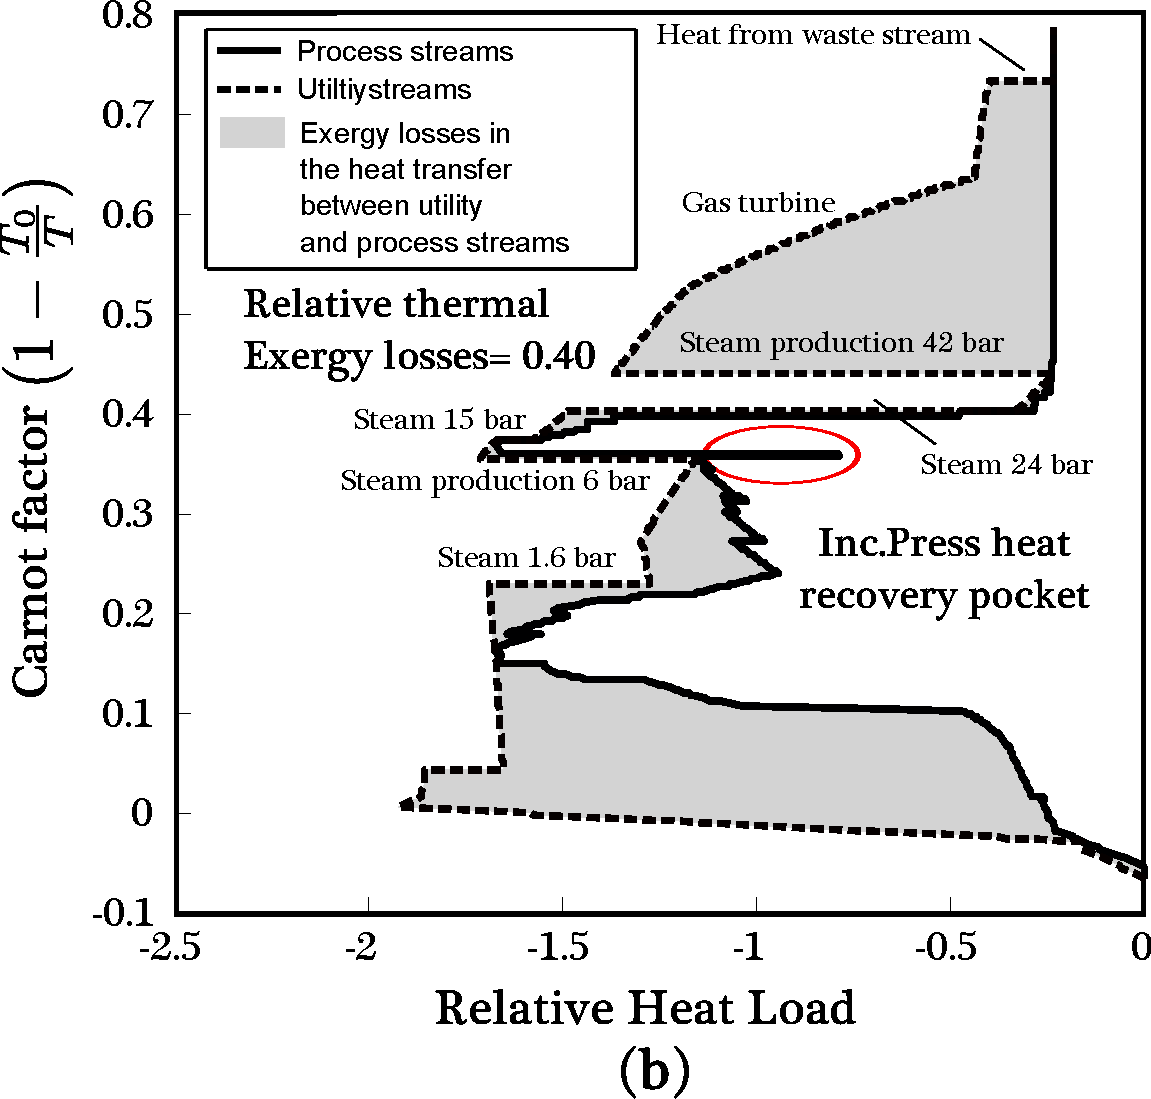
\includegraphics[width=70mm]{images/ch3/figutilityb.pdf}
 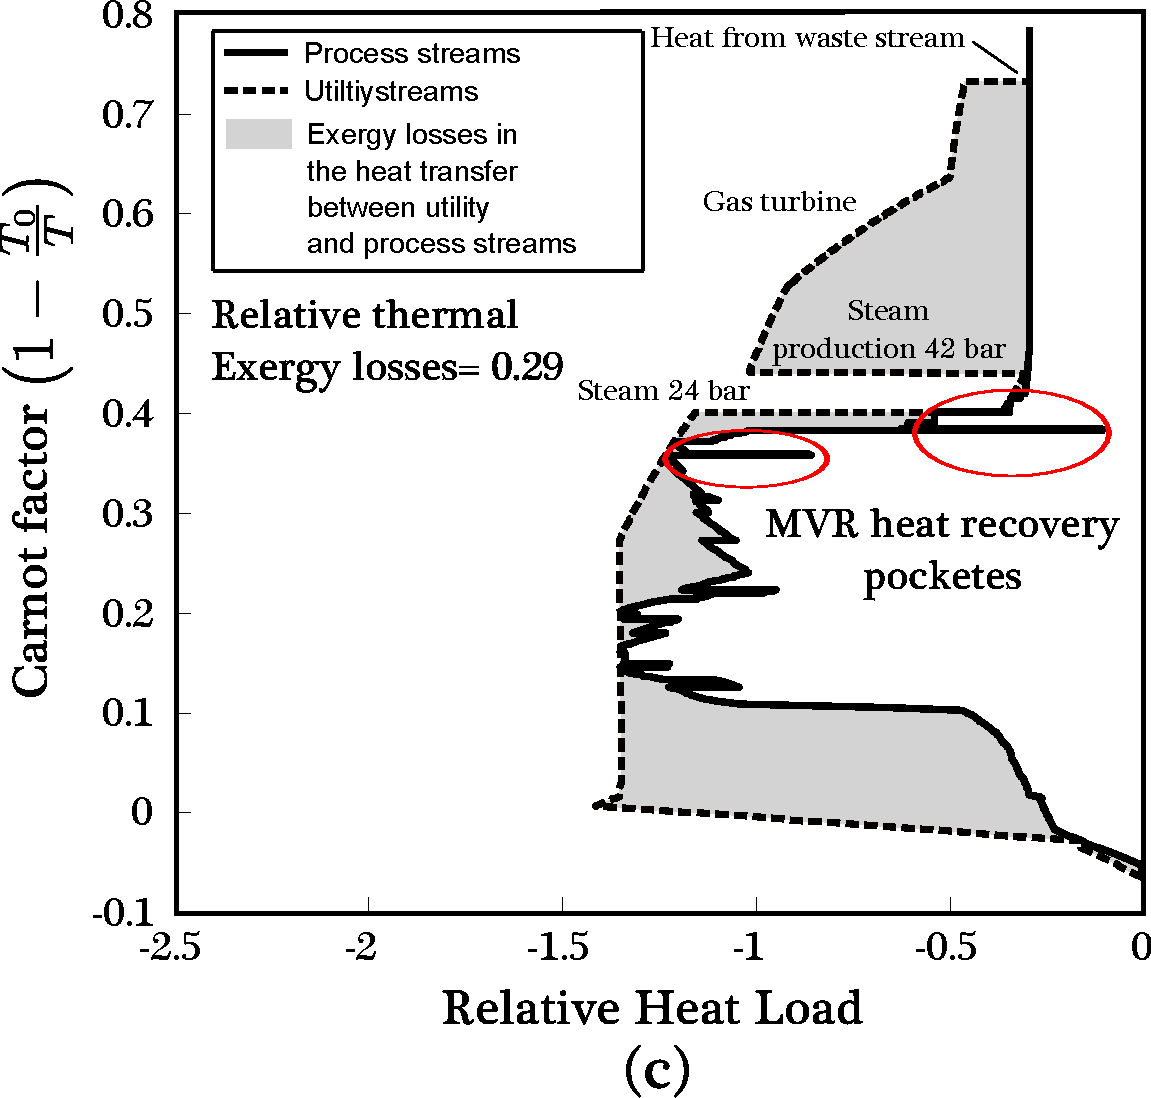
\includegraphics[width=70mm]{images/ch3/figutilityc.pdf}
 \caption{Site utility integration and optimization for three different scenarios}
 \label{fig3:VIIII}
 \end{center}
  \vspace{-5mm}
 \end{figure}
 
 The proposed solutions are simplified based on both technical feasibilities and the preference of the plant, even if there were a further possibility to produce electricity by the cogeneration unit and through improvement of the steam network. The finalized solutions are then evaluated based on the operating and investment cost and are also compared to the current situation of the plant. The investment cost includes the one required to purchase new equipments, such as the heat exchangers, compressors and turbines. The summary of the analysis is presented in \cref{tab3:two}. The reported relative electricity balance is using the current natural gas consumption as a reference and is positive when electricity is exported. It accounts only for the utility system balance and does not include electricity consumption of the processes. The relative annualized investment cost similarly is using the current annual operating cost as the reference. For the estimation of the investment cost, standard techniques have been used. 
 
 \label{tab3:two}
 
 This analysis shows that the natural gas and electricity consumption have been reduced in each scenario. 
Since the current site uses a simple boiler, installation of a cogeneration system slightly increases the natural gas consumption, simultaneously satisfying MER and producing electricity. However, the total cost of the TSI scenario is reduced considerably by 22\% due to the cogeneration and heat recovery effects. The reduction of gas consumption in the scenario with MVR and heat pumps reaches 40\%, but its effect on the total cost is only 30\% due to the electricity consumption of MVR system and its higher investment cost.
 
 
